\chapter{Denial of Service Testing}

	The most common type of denial of service (DoS) attack is the kind used on a network to make 
	a server unreachable by other valid users. The fundamental concept of a network DoS attack 
	is a malicious user flooding enough traffic to a target machine, that it renders the target 
	incapable of keeping up with the volume of requests it is receiving. 

	\section{Testing for SQL Wildcard Attacks}

	SQL Wildcard Attacks are about forcing the underlying database to carry out CPU-intensive queries 
	by using several wildcards. This vulnerability generally exists in search functionalities of web
	applications. Successful exploitation of this attack will cause Denial of Service.
	SQL Wildcard attacks might affect all database back-ends but mainly affect SQL Server because the 
	MS SQL Server {\bf LIKE operator} supports extra wildcards.

	Craft a query which will not return a result and includes several wildcards. You can use one of 
	the example inputs below. Send this data through the search feature of the application. If the 
	application takes more time generating the result set than a usual search would take, it is 
	vulnerable.

	\begin{figure}[H]
		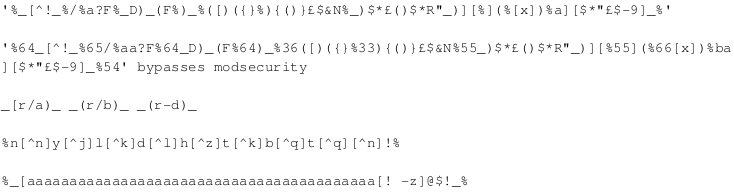
\includegraphics[width=\textwidth]{pics/DOS1.png}
	\end{figure}

	{\bf How to craft search strings for testing:} \\
		\begin{itemize}
			\item Queries should return as few results as possible or even none at all. 
			In this way, we can be sure that we actually forced the database server to search all records.
			\item During the OR combinations, every OR statement should be different, otherwise the 
			database will optimize it. Changing one character is enough.
			\item  In Microsoft SQL Server, every character after an open bracket [ causes unusually 
			long execution time. 
			\item Longer queries will generally result in longer execution time. Craft the longest 
			possible query allowed by the application.
			\item Starting with \% and ending with \% will generally cause longer running queries.
			\item Some search implementations may cache search results. During the testing, every
			search query should be slightly different to avoid this.
			\item Performance is always about experimenting. Try different combinations to find the 
			most expensive queries for that particular target system and data.
		\end{itemize}

	\section{Locking Customer Accounts}
		In this test we check whether an attacker can lock valid user accounts by repeatedly attempting 
		to log in with a wrong password. The first test that must be performed is to test that an account 
		does indeed lock after a certain number of failed logins. To determine valid account names, a 
		tester should look to find places where the application discloses the difference between valid and
		invalid logins. Common places this would occur are:
			\begin{itemize}
				\item {\bf The login page} – Using a known login with a bad password, look at the error message
				returned to the browser.
				\item {\bf New account creation page} – If the application allows people to create a new
				account that includes the ability to choose their account name, it may be possible to discover 
				other accounts in this manner. What happens if you try to create a new account using an
				account name that is already known to exist? 
				\item {\bf Password reset page} – If the login page also has a function for recovering or 
				resetting a password for a user, look at this function as well. Does this function 
				give different messages if you attempt to reset or recover an account that does not exist in 
				the system?
			\end{itemize}

	\section{Buffer Overflows}

		Any language where the developer has direct responsibility for managing memory allocation, 
		most notably C and C++, has the potential for a buffer overflow. 

		The following is a simplified example of vulnerable code in C:

		\begin{figure}[H]
			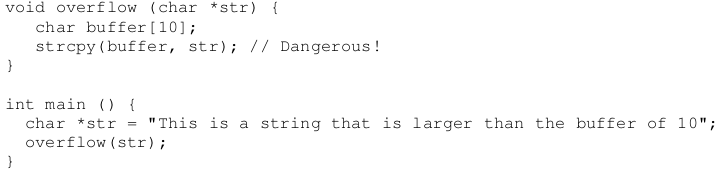
\includegraphics[width=\textwidth]{pics/buffer.png}
		\end{figure}

		If this code example were executed, it would cause a segmentation fault and dump core. 
		The reason is that strcpy would try to copy 53 characters into an array of 10 elements 
		only, overwriting adjacent memory locations. 

	\section{User Input As a Loop Counter}

		In this test we check whether it is possible to force the application to loop through a 
		code segment that needs high computing resources, in order to decrease its overall 
		performance. Like the previous problem of User Specified Object Allocation, if the user 
		can directly or indirectly assign a value that will be used as a counter in a loop function, 
		this can cause performance problems on the server. The following is an example of vulnerable 
		code in Java:
	
		\begin{figure}[H]
			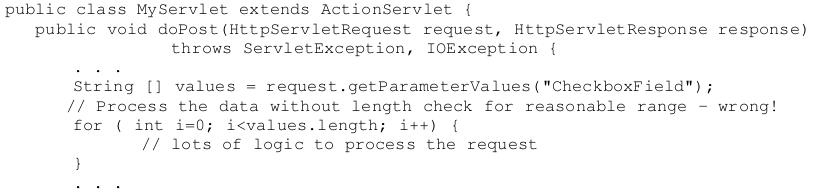
\includegraphics[width=\textwidth]{pics/loop.png}
		\end{figure}

		As we can see in this simple example, the user has control over the loop counter. If the code 
		inside the loop is very demanding in terms of resources, and an attacker forces it to be executed 
		a very high number of times, this might decrease the performance of the server in handling other
		requests, causing a DoS condition.

	\section{Failure to Relese Resources}
		With this test, we check that the application properly releases resources (files and/or memory) 
		after they have been used.

		Possible examples include:
			\begin{itemize}
				\item An application {\bf locks a file for writing}, and then an exception occurs but does 
				not explicitly close and unlock the file.
				\item {\bf Memory leaking} in languages where the developer is responsible for memory 
				management such as C and C++. 
				\item Use of {\bf DB connection} objects where the objects are not being freed if 
				an exception is thrown. A number of such repeated requests can cause the application 
				to consume all the DB connections, as the code will still hold the open DB object, 
				never releasing the resource.
			\end{itemize}

		The following is an example of vulnerable code in Java. In the example, both the Connection and 
		the CallableStatement should be closed in a finally block.

		\begin{figure}[H]
			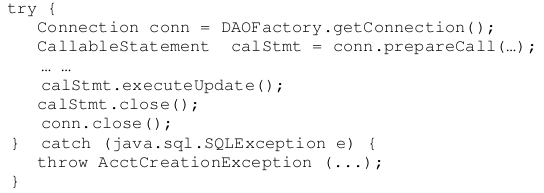
\includegraphics[width=\textwidth]{pics/DBConnection.png}
		\end{figure}

		






